\documentclass[12pt,oneside,openany,a4paper, %... Layout
afrikaans,english,
%... Global lang drivers
]{memoir}
\usepackage[report, goldenblock]{usthesis}%... Thesis options
\usepackage[afrikaans, english]{babel}
%\SingleSpacing
\usepackage[left=3cm, right=2cm, top=2.5cm, bottom=2.5cm]{geometry}
\usepackage{amsmath}
\usepackage{mathtools}
\numberwithin{equation}{chapter}
\usepackage{bm}
\usepackage{graphicx}
\usepackage{subcaption}
\usepackage{color} % or xcolor
\usepackage{float} %figure location

\renewcommand{\thesection}{\thechapter.\arabic{section}}
\usepackage{tabto}

%Watermark
\usepackage{eso-pic}
\newcommand*{\WaterMark}[2][0.15\paperwidth]{%
\AddToShipoutPicture*{\AtTextCenter{%
\parbox[c]{0pt}{\makebox[0pt][c]{%
\includegraphics[width=#1]{#2}}}}}}

%References
\usepackage{usbib}%............................. Bibliography
\bibliographystyle{usmeg-n}%................. Auhor-year style
\addto{\captionsenglish}{\renewcommand{\bibname}{List of References}}

\begin{document}
\pagestyle{plain}
\frontmatter
%TiltePage:
\title{Numerical integration for probabilisitc reasoning skripsie}
\author{JM.\ Louw}{Jacobus Martin Louw}
\faculty{Faculty of Electrical and Electronic Engineering}
\degree{BEng (E&E)}{Bachelor of Engineering (Electrical and Electronic)}
\ReportDescript{Final Report}
\supervisor{Dr\ CE\ van Daalen}
\frontmatter
\WaterMark{UScrest-WM}
\TitlePage

\addtocontents{toc}{\protect\setcounter{tocdepth}{-1}}
%Declaration Page
\DeclarationPage

%abstract
\address{Department of Electrical and Electronic Engineering,\\
University of Stellenbosch,\\
Private Bag X1, 7602 Matieland, South Africa.}
\newpage

\tableofcontents
\addtocontents{toc}{\protect\setcounter{tocdepth}{2}}
\pagebreak
\listoffigures

\chapter{List of Acronyms}
RV -	random variable\\
PGM		-	probabilistic graphical model\\
PDF		-	probability density function\\
CPD		-	conditional probability distribution\\
KF		-	Kalman Filter\\
EKF		-	Extended Kalman Filter\\
UKF		-	Unscented Kalman Filter\\

\begin{abstract}
Text in default language ...
\end{abstract}


\mainmatter
\chapter{Introduction}
Robot localisation is the process of estimating where a robot is located relative to its environment. It is essential for autonomous robots to have precise knowledge of their location in order to navigate their surroundings.\\
When localising a robot, the control input to the robot, and a map of the environment is usually available. Further the robot is generally fitted with sensors which, together with beacons, measure where the robot is located relative to the map. Unfortunately the information of the robot's movements and location always have noise to some degree.\\
The position and orientation of the robot should rather be estimated in a probabilistic manner from the information gathered from the sensors. The localisation techniques must therefore be able to deal with noise and describe the robot's location with a measure of uncertainty.\\
Probabilistic reasoning of systems with continuous random variables (RV) use integration for various operations. In most nonlinear systems these integrals cannot be calculated analytically and one must use numerical methods. Kalman filters have been used extensively to localise robots and other objects. Techniques such as the extended or unscented Kalman filters use primitive numerical integration that is very inaccurate, especially when measurements are also nonlinear. However, there are several alternative numerical techniques available that are more accurate.\\
A probabilistic graphical model (PGM) is a technique that is be used to model systems with uncertainty in an organised manner. It describes the relationship between random variables (RV) and allows to reason about their likelihood based on knowledge that is available to the system. Reasoning about RVs in a PGM consists out of concrete steps and one can easily identify where integration is used.\\
The end goal of this project is investigate different numerical techniques of integration and to implement them in a PGM to localise a simulated robot. The accuracy and efficiency of different techniques of numerical integration when used to inference a nonlinear system will be compared using a simulated environment.
\setcounter{secnumdepth}{2}
\chapter{Gaussian Random Variables}
The Gaussian or normal distribution is commonly used in probability theory, as it is very easy to work with. Although Gaussian distributions make severe assumptions such as exponential decay of the distribution away from its mean and linear interactions between variables, they are often surprisingly good estimations for real world distributions, such as noise. The Gaussian distribution is a very important concept in this report as all probability distributions are approximated as Gaussian distributions. Key concepts and features of the Gaussian distributions are discussed in this chapter. The canonical form and conditional distributions are very important concepts and will be used in following chapters. The following chapter is based on the work of Peebles and Shi~\cite{peebles} and Koller and Friedman~\cite{koller}.

\section{Covariance form}
The likelihood of the values of a continuous Gaussian RV can be described with a Gaussian distribution. \
The univariate Gaussian distribution is probability density function (PDF) of a single Gaussian RV. The covariance form fully describes a univariate Gaussian distribution by a mean $\mu$ and variance $\sigma^2$.
The univariate Gaussian distribution of a RV $X$, denoted
\begin{equation}
X\sim\mathcal{N}(\mu,\sigma),
\end{equation}
has a PDF that is described by
\begin{equation}\label{eq:1}
p(x) = \eta\exp\left[\frac{-(x-\mu)^2}{2\sigma^2}\right],
\end{equation}
with a normalisation coefficient 
\begin{equation}\label{eq:2}
\eta = \frac{1}{\sqrt{2\pi\sigma^2}}.
\end{equation}
The mean parameter $\mu$ describes the location of the peak of the distribution and the variance parameter $\sigma^2$ describes the tempo which the distribution decays. The probability of RV $X$ having a value $x$ decays exponentially as $x$ moves farther from the mean. The standard deviation of the Gaussian distribution is denoted as $\sigma$.\\
If $X$ is a continuous RV, then the mean or expectation of $X$ is
\begin{equation}
\mu = E\left[ X \right] = \int x \cdot p(x)dx.
\end{equation}
The variance of $X$ can be calculated as
\begin{equation}
\sigma^2 = E[X^2] - (E[X])^2
\end{equation}
 Figure \ref{fig:gPDF1} indicates the mean $\mu$ and standard deviation $\sigma$ of an univariate Gaussian PDF.
\begin{figure}[H]
  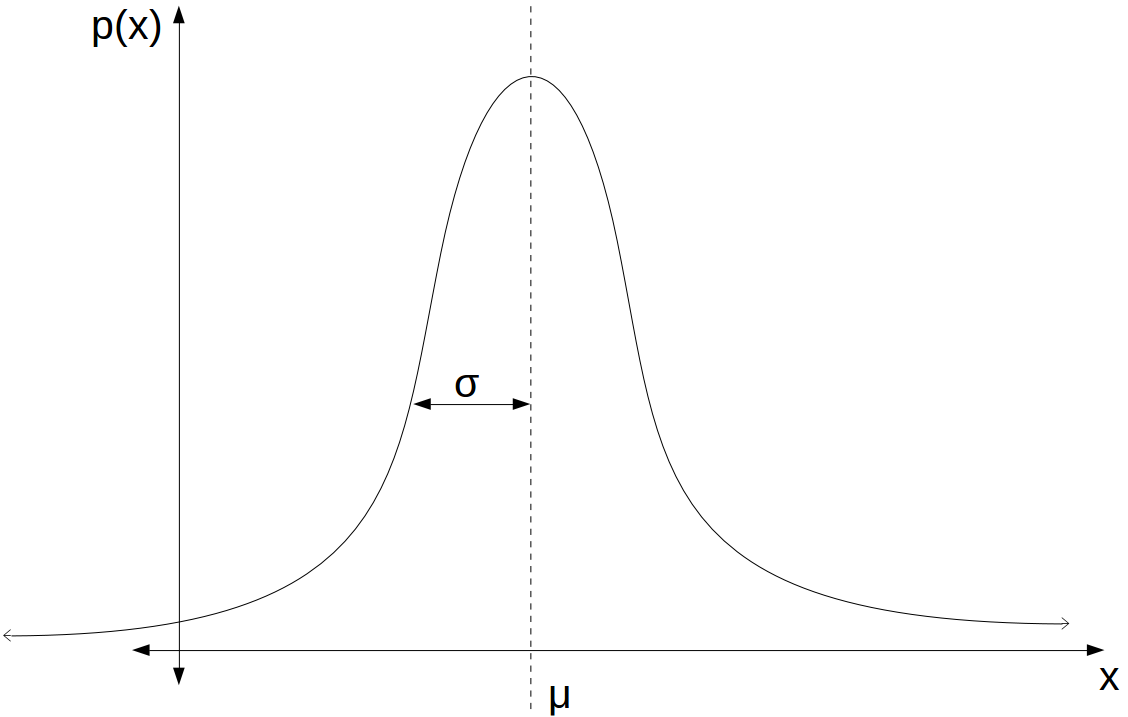
\includegraphics[width=0.6\linewidth]{Figures/univariate.png}
  \centering
  \caption{Univariate Gaussian PDF}
  \label{fig:gPDF1}
\end{figure}
The definition of the Gaussian distribution can be extended to describe the PDF of $N$ random variables, this is called the multivariate Gaussian distribution. The multivariate Guassian distribution is described by an $N$-dimensional mean vector $\bm{\mu}$ and an $N\times N$ covariance matrix $\Sigma$. The multivariate Gaussian distribution of a RV vector a with length of $N$, $\bm{X} = [X_1,...,X_N]$, denoted
\begin{equation}
\bm{X} \sim \mathcal{N}(\bm{\mu},\Sigma),
\end{equation}
has a PDF that is described by
\begin{equation}\label{eq:3}
p(\bm{x})  = \eta\exp\left[-\frac{1}{2}(\bm{x}-\bm{\mu})^T\Sigma^{-1}(\bm{x}-\bm{\mu})\right],
\end{equation}
with a normalisation coefficient
\begin{equation}\label{eq:4}
\eta = \frac{1}{(2\pi)^{\frac{N}{2}}|\Sigma|^{\frac{1}{2}}}.
\end{equation}
$|\Sigma|$ is the the determinant of $\Sigma$.\\
For this report it is required that $\Sigma$ is positive definite and thus also non-singular, which guarantees a determinant that is nonzero. Positive definite covariance matrices are also invertible, thus the alternative canonical or information parameterization, which requires $\Sigma^{-1}$, can be used. The canonical form is discussed in the following section.\\
The mean vector of RV vector $\bm{X}$ is equal to the expectation of $\bm{X}$ and is defined as
\begin{equation}
\bm{\mu} = E[\bm{X}].
\end{equation}
The covariance matrix $\Sigma$ specifies the correlation between RVs and is equal to
\begin{equation}
\Sigma = E[\bm{XX}^T] - E[\bm{X}]\bm{E}[\bm{X}]^T.
\end{equation}
\subsection{Error ellipse}The following section is based on an article by H. Abdi ~\cite{abdi} and on a webpage from "Computer vision for dummies"~\cite{draw_ellipse}.\par
A multivariate Gaussian distribution with RV vector
\begin{equation}
\bm{X} = [X_1, X_2]
\end{equation}
can be visualised as a series of ellipsoidal contours around the mean vector $\bm{\mu}$. The contours are an indication of the correlation between $X_1$ and $X_2$ and also show the uncertainty of the PDF. Contours close to each other suggest a steep incline and contours farther apart suggest a gradual incline in the PDF. Hence, small and concentrated contours represent certain Gaussian distributions and contours that are larger and further apart represent uncertain Gaussian distributions. Error ellipsis are an effective way to indicate the mean, uncertainty and correlation of 2D Gaussian distributions.

An ellipse has a major axis and a minor axis as shown in Figure \ref{fig:e_ellipse}. The major axis of the error ellipse is always aligned in the direction the Gaussian distribution varies most. This direction can be found by determining the eigenvectors of the distribution. Each eigenvector has a corresponding eigenvalue which indicates the spread of the distribution in the direction of the eigenvector. 

We can use eigenvalue decomposition to factorise the covariance matrix $\Sigma$,
\begin{equation}
\Sigma = Q\Lambda Q^{-1}.
\end{equation}
Each column of the eigenvector matrix $Q$ contains an eigenvector $\bm{v}$. $Q$ is defined as
\begin{equation}
Q =
[\bm{v_1} \ \bm{v_2}]
=
\begin{bmatrix}
v_{11} & v_{21}\\
v_{12} & v_{22}
\end{bmatrix}.
\end{equation}
$\Lambda$ is a diagonal matrix and each of its diagonal entries contains an eigenvalue $\lambda$. $\Lambda$ is defined as 
\begin{equation}
\Lambda =
\begin{bmatrix}
\lambda_1 & 0\\
0 & \lambda_2
\end{bmatrix}.
\end{equation}
An error ellipsis of a Gaussian PDF can be specified in terms of confidence levels which is the probability that a value drawn from the distribution will fall inside the ellipse. Thus, differently sized ellipsis can be plotted for different confidence levels. The lengths of the major an minor axes are sequentially specified as $2\sqrt{s\lambda_1}$ and $2\sqrt{s\lambda_2}$, where $\lambda_1 \geq \lambda_2$. The value of $s$ is determined by the confidence level of the error ellipse. In the case of an error ellipse with a confidence level of 95\%, $s$ is set to 5.991. The Chi-Sqaure distribution can be used to find $s$ for other confidence levels, but it is beyond the scope of this document.

The orientation $\alpha$ of the error ellipse is shown in Figure \ref{fig:e_ellipse}. To obtain $\alpha$ we calculate the angle, relative to the x-axis, of the eigenvector with the largest spread. The angle $\alpha$ is defined as
\begin{equation}
\alpha = \arctan\left(\frac{v_{11}}{v_{12}}\right),
\end{equation}
where $\lambda_1 \geq \lambda_2$.

\begin{figure}[H]
  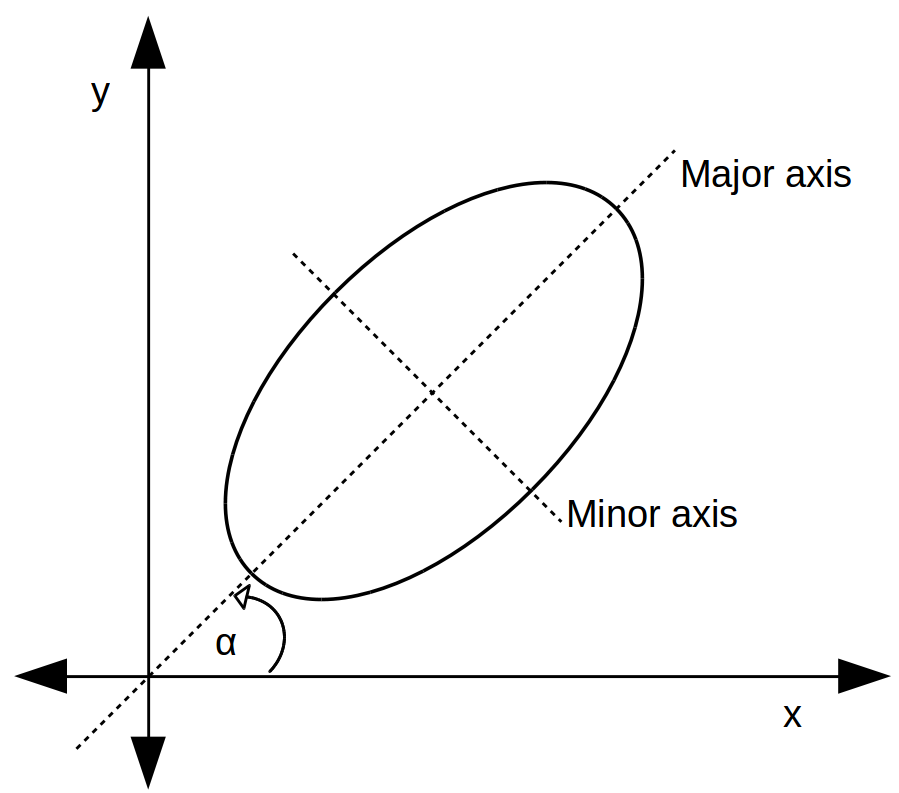
\includegraphics[width=0.5\linewidth]{Figures/e_ellipse.png}
  \centering
  \caption{Error Ellipse}
  \label{fig:e_ellipse}
\end{figure}
\section{Canonical form}
The canonical or information form is an alternative way to represent Gaussian distributions. A big advantage of using the canonical form is that it is much easier to perform certain operations. It can also be used to represent Gaussina conditional probability densities (CPDs), which will be discussed later in this section. The following section is based on the work of Koller and Friedman~\cite{koller} and Schoeman~\citep{JC}.

Equation \ref{eq:3}, which is the definition of a Gaussian PDF, can be rewritten
\begin{equation}
\begin{split}\label{eq:6}
p(\bm{x}) & = \eta\exp\left[-\frac{1}{2}(\bm{x}-\bm{\mu})^T\Sigma^{-1}(\bm{x}-\bm{\mu})\right]\\
& = \exp\left(-\frac{1}{2}\bm{x}^T\Sigma^{-1}\bm{x} + \bm{\mu}^T\Sigma^{-1}\bm{x} - \frac{1}{2}\bm{\mu}^T\Sigma^{-1}\bm{\mu} + \ln{\eta}\right),
\end{split}
\end{equation}
with the information matrix
\begin{equation}\label{eq:7}
K = \Sigma^{-1},
\end{equation}
the potential vector
\begin{equation}\label{eq:8}
\bm{h} = \Sigma^{-1}\bm{\mu},
\end{equation}
and
\begin{equation}\label{eq:9}
g = - \frac{1}{2}\bm{\mu}^T\Sigma^{-1}\bm{\mu} + \ln{\eta}.
\end{equation}
Thus the definition of the canonical form is
\begin{equation}\label{eq:canonical}
\mathcal{C}(\bm{x}; K,\bm{h},g) = \exp\left(-\frac{1}{2}\bm{x}^TK\bm{x} + \bm{h}^T\bm{x} +g \right).
\end{equation}
As one can always determine $g$ from $\bm{h}$ and $K$, thus a more general notation for a Gaussian distribution in canonical form is $\mathcal{C}(\bm{x}; K,\bm{h})$.

It is easy to recover the covariance parameters:
\begin{equation}
\Sigma = K^{-1}
\end{equation}
\begin{equation}
\bm{\mu} = \Sigma\bm{h}
\end{equation}
Sometimes $K$ is not invertible and the covariance can not be recovered, the canonical form is therfore more general than the covariance form.

It can be seen from the above that it is very easy to switch between the canonical an covariance form. 
\subsection{Operations using the canonical form}
A big advantage of using the canonical form is that it makes it easy to perform various operations on Gaussian distributions. This section will cover useful operations using the canonical form. 

Extending and rearranging scopes of canonical forms may be necessary before doing operations, as it is important that scopes of canonical forms are identical when doing operations. 
\subsubsection{Extending the scope of a canonical form:}
The scope of a canonical form can be extended by adding zero entries to $K$ and $\bm{h}$:
\begin{equation}
\mathcal{C}\left(
\begin{bmatrix}
x\\
y
\end{bmatrix};
\begin{bmatrix}
k_{xx} & k_{xy}\\
k_{yx} & k_{yy}
\end{bmatrix},
\begin{bmatrix}
h_x\\
h_y
\end{bmatrix}
\right)
=
\mathcal{C}\left(
\begin{bmatrix}
x\\
y\\
z
\end{bmatrix};
\begin{bmatrix}
k_{xx} & k_{xy} & 0\\
k_{yx} & k_{yy} & 0\\
0 & 0 & 0
\end{bmatrix},
\begin{bmatrix}
h_x\\
h_y\\
0
\end{bmatrix}
\right)
\end{equation}
\subsubsection{Rearranging the scope of a canonical form:}
The scope can be rearranged by rearranging the rows and columns of $K$  and rearranging the entries of $\bm{h}$:
\begin{equation}
\mathcal{C}\left(
\begin{bmatrix}
x\\
y\\
z
\end{bmatrix};
\begin{bmatrix}
k_{xx} & k_{xy} & k_{xz}\\
k_{yx} & k_{yy} & k_{yz}\\
k_{zx} & k_{zy} & k_{zz}
\end{bmatrix},
\begin{bmatrix}
h_x\\
h_y\\
h_z
\end{bmatrix}
\right)
=
\mathcal{C}\left(
\begin{bmatrix}
y\\
x\\
z
\end{bmatrix};
\begin{bmatrix}
k_{yy} & k_{yx} & k_{yz}\\
k_{xy} & k_{xx} & k_{xz}\\
k_{zy} & k_{zx} & k_{zz}
\end{bmatrix},
\begin{bmatrix}
h_y\\
h_x\\
h_z
\end{bmatrix}
\right)
\end{equation}
\subsubsection{Multiplication of canonical forms:}
If the scopes of two canonical forms are identical, one can multiply them by simply summing the $K$ and $\bm{h}$ parameters:
\begin{equation}\label{eq:10}
\mathcal{C}(K_1,\bm{h_1},g_1)\times\mathcal{C}(K_2,\bm{h_2},g_2) = \mathcal{C}(K_1 + K_2,\bm{h_1} + \bm{h_2},g_1 + g_2)
\end{equation}
%\subsubsection{Division of canonical forms:}
%Again, it important that the scopes of the distributions are identical.
%\begin{equation}\label{eq:11}
%\frac{\mathcal{C}(K_1,\bm{h_1},g_1)}{\mathcal{C}(K_2,\bm{h_2},g_2)} = %\mathcal{C}(K_1 - K_2,\bm{h_1} - \bm{h_2},g_1 - g_2)
%\end{equation}
\subsubsection{Marginalisation of a canonical form:}
A marginal distribution can be found by integrating over a subset of variables. For example the marginal distribution over $\bm{x}$ can be found by integrating over $\bm{y}$. Let $\mathcal{C}(\bm{x},\bm{y};K,\bm{h},g)$ be a canonical form with subsets $\bm{x}$ and $\bm{y}$ where
\begin{equation}
K = 
\begin{bmatrix}
K_{\bm{xx}} & K_{\bm{xy}}\\
K_{\bm{yx}} & K_{\bm{yy}}
\end{bmatrix}
 ;\ h = 
\begin{pmatrix}
h_{\bm{x}} \\
h_{\bm{y}}
\end{pmatrix}.
\end{equation}
To obtain the marginal distribution over $\bm{x}$, we have to find the integral over $\bm{y}$. Therefore the marginal distribution over $\bm{x}$ is
\begin{equation}
\int\mathcal{C}(\bm{X},\bm{Y};K,\bm{h},g)d\bm{Y} = \mathcal{C}(\bm{X};K',\bm{h}',g'),
\end{equation}
 where
\begin{equation}
K' = K_{\bm{xx}} - K_{\bm{xy}}K_{\bm{yy}}^{-1}K_{\bm{yx}},
\end{equation}
\begin{equation}
h' = \bm{h}_{\bm{x}} - K_{\bm{xx}}K_{\bm{yy}}^{-1}\bm{h}_{\bm{y}},
\end{equation}
and
\begin{equation}
g' = g - \frac{1}{2}\left(\ln|2\pi K_{\bm{yy}}^{-1}|+ \bm{h_y}^T K_{\bm{yy}}^{-1}\bm{h_y}\right).
\end{equation}
It is important to that $K_{\bm{yy}}$ is positive-definite for the result to be finite.
\subsubsection{Reduction with evidence:}
Let $\mathcal{C}(\bm{X},\bm{Y};K,\bm{h},g)$ be a canonical form with subsets $\bm{X}$ and $\bm{Y}$. If subset $\bm{Y}$ is known $(\bm{Y} =  \bm{y})$, then the canonical form can be reduced to $\mathcal{C}(\bm{X}; K',\bm{h}',g')$, where
\begin{equation}
K' = K_{\bm{XX}}
\end{equation}
\begin{equation}
h' = \bm{h}_{\bm{X}} - K_{\bm{XY}}\bm{y}
\end{equation}
\begin{equation}
g' = g + \bm{h}_{\bm{Y}}^T\bm{y} - \frac{1}{2}\bm{y}^TK_{\bm{YY}}\bm{y}
\end{equation}
\subsection{Using the canonical form the present conditional distributions (linear transformations)}
The following section is based on a skripsie from JC Schoeman~\cite{JC} and notes from Dr CE van Daalen. One of the advantages of the canonical form is that it is possible to present conditional probability distributions (CPDs). \\
If a CPD such as $p(\bm{y}|\bm{x})$ can be described as a linear transform:
\begin{equation}
\bm{y} = F\bm{x} + \bm{g} + \bm{n}
\end{equation}
where
\begin{equation}
n = \mathcal{N}(\bm{0}, \Sigma_n)
\end{equation}
\begin{equation}
\label{eq:30}
\begin{split}
p(\bm{y}|\bm{x}) & = \mathcal{N}(F\bm{x} + \bm{g}, \Sigma) \\
& = \eta\exp\left[-\frac{1}{2}(\bm{y} - (F\bm{x} + \bm{g}))^T\Sigma^{-1}(\bm{y}-(F\bm{x} + \bm{g}))\right]
\end{split}
\end{equation}
Rewriting
\begin{equation}
\begin{split}
\bm{y} - (F\bm{x} + \bm{g}) & =
\begin{bmatrix}
I&-F&-I
\end{bmatrix}
\begin{bmatrix}
\bm{y}\\
\bm{x}\\
\bm{g}
\end{bmatrix}\\
& =
\begin{bmatrix}
I\\-F^T\\-I
\end{bmatrix}^T
\begin{bmatrix}
\bm{y}\\
\bm{x}\\
\bm{g}
\end{bmatrix}\\
\end{split}
\end{equation}
Equation \ref{eq:30} becomes
\begin{equation}
\label{eq:32}
\begin{split}
p(\bm{y}|\bm{x}) = \eta\exp\left[-\frac{1}{2}
\begin{bmatrix}
\bm{y}\\
\bm{x}\\
\bm{g}
\end{bmatrix}^T
\begin{bmatrix}
I\\-F^T\\-I
\end{bmatrix}
\Sigma^{-1}
\begin{bmatrix}
I\\-F^T\\-I
\end{bmatrix}^T
\begin{bmatrix}
\bm{y}\\
\bm{x}\\
\bm{g}
\end{bmatrix}
\right]
\end{split}
\end{equation}
Defining a combined random vector
\begin{equation}
\bm{w} = 
\begin{bmatrix}
\bm{y}\\
\bm{x}\\
\bm{g}

\end{bmatrix}
\end{equation}
and information matrix
\begin{equation}
K' =
\begin{bmatrix}
I\\-F^T\\-I
\end{bmatrix}
\Sigma^{-1}
\begin{bmatrix}
I\\-F^T\\-I
\end{bmatrix}^T
\end{equation}
Equation \ref{eq:32} can be rewritten
\begin{equation}
\label{eq:35}
\begin{split}
p(\bm{y}|\bm{x}) = \eta\exp\left[-\frac{1}{2}
\bm{w}^T
K'
\bm{w}
\right]
\end{split}
\end{equation}
This closely relates with the canonical form in equation \ref{eq:canonical}
\begin{equation}
\begin{split}
p(y|x) & = \mathcal{C}(\bm{w}: K', \bm{0})\\
& =\mathcal{C}\left(
\begin{bmatrix}
\bm{y} \\
\bm{x} \\
\bm{g}
\end{bmatrix};
\begin{bmatrix}
I\\
-F^T\\
-I
\end{bmatrix}
\Sigma_n^{-1}
\begin{bmatrix}
I & -F & -I
\end{bmatrix}, \bm{0}, -
\right)\\
& =\mathcal{C}\left(
\begin{bmatrix}
\bm{y} \\
\bm{x} \\
\end{bmatrix};
\begin{bmatrix}
I\\
-F^T
\end{bmatrix}
\Sigma_n^{-1}
\begin{bmatrix}
I & -F
\end{bmatrix},
\begin{bmatrix}
I\\
-F^T
\end{bmatrix}
\Sigma_n^{-1}\bm{g}, -
\right)\\
& =\mathcal{C}\left(
\begin{bmatrix}
\bm{y} \\
\bm{x} \\
\end{bmatrix};
\begin{bmatrix}
\Sigma_n^{-1}  &  -\Sigma_n^{-1}F\\
-F^T\Sigma_n^{-1} & F^T\Sigma_n^{-1}F
\end{bmatrix}
, 
\begin{bmatrix}
-\Sigma_n^{-1}\bm{g}\\
-F^T\Sigma_n^{-1}\bm{g}
\end{bmatrix},
-
\right)
\end{split}
\end{equation}
\chapter{Motion models}
Before implementing a localisation algorithm to localise an object, it is important to have a model which desctibes the movement of the object. A simple linear motion model will be covered which will later be used to illustrate basic principles when localising linear moving objects. A more sophisticated nonlinear motion model will be explored which will be essential when investigating numerical integration techniques for localising nonlinear moving objects. This chapter is based on the work of S. Thrun, W. Burgard and D. Fox~\citep{thrun};
\section{Basic concepts}
The motion model describes $p(x_t|u_t,x_{t-1})$, which is the transition probability and it is vital in the the prediction step of the Bayes filter. The material will cover kinematics in a stochastic form. Robot motion will be limited to planar movement as it is easier to convey concepts or ideas to the reader. Note that the theory discussed is not limited to planar movement.  
\section{Linear Motion}

\section{Nonlinear motion}
\subsection{Velocity motion model}
\chapter{Localisation using Kalman Filters}
This chapter will focus on localisation using traditional techniques such as the Kalman filter, extended Kalman filter and Unscented Kalman filter. This is important to investigate and understand as there is a strong correspondance to the PGM technique that will be discussed in a following section. The motion an measurement models will also be discussed 
\section{Motion models}
\section{Measurement models}
\section{Kalman Filter}
\section{Extended Kalman Filter}
\section{Unscented Kalman Filter}
\chapter{Probabilistic Graphical Models}
This chapter gives a brief introduction to Probabilistic Graphical Models (PGMs). PGMs are a very vast field which is beyond the scope of this document, therefore only the theory relevant to this paper will be covered. This chapter is based on the work of Koller and Friedman~\cite{koller}, Barber~\cite{barber} and Schoeman~\citep{JC}.
\section{Overview}
Reasoning about systems with uncertainty can become very complex and sometimes it is completely unmanageable. The PGM is a graphical technique which allows to model probabilistic systems in a logical and compact manner which makes problems tractable. PGMs are thus used to describe the relationship between RVs and allows to reason about them. This action of querying a system or reasoning about a variable is called inference. The relationships in a PGM are usually in the form of conditional probability densities (CPDs). It is a very popular technique, as it is intuitive, transparent and easy to manipulate. Hence, PGMs have countless applications from making medical diagnosis to localising robots. Although it is a powerful technique, it has its limitations such as image recognition, where neural networks thrive.\\
PGMs can be divided in to two categories. The first is Markov networks, which are used for non-causal systems, and the second is Bayesian networks, which are used for causal systems. As the localisation problem is in most cases causal, the focus of this chapter is on Bayesian networks.\\
The theory is also discussed in terms of continuous RVs, because problems addressed in following chapters make use of continuous RVs. Note that all of the theory can also be applied to discrete RVs. 
\section{Basic concepts of graphical models}
A graph consists of nodes and edges. Edges are the link between nodes and can be directed or undirected. If all edges are undirected then the graph is classified as undirected. If all edges are directed, then the graph is classified as directed. Bayesian networks are directed and Markov networks are undirected.\\
In the case of directed graphs, nodes can be classified as ancestors, parents, children and descendants. If there exists a directed path from $X_1 \to X_k$, then $X_1$ is an ancestor of $X_k$, and $X_k$ is a descendant of $X_1$. In Figure \ref{fig:comGraphs}(b), $a$ is an ancestor of $c$ and $c$ is a descendant of $a$. A parent is an ancestor with only one edge between the ancestor and descendant. A child is a descendant with only one edge between the descendant and the ancestor. In Figure \ref{fig:comGraphs} (b), then $a$ is a parent of $b$ and $b$ is a child of $a$.~\cite{barber}
\begin{figure}[h!]
  \centering
  \begin{subfigure}[b]{0.3\linewidth}
    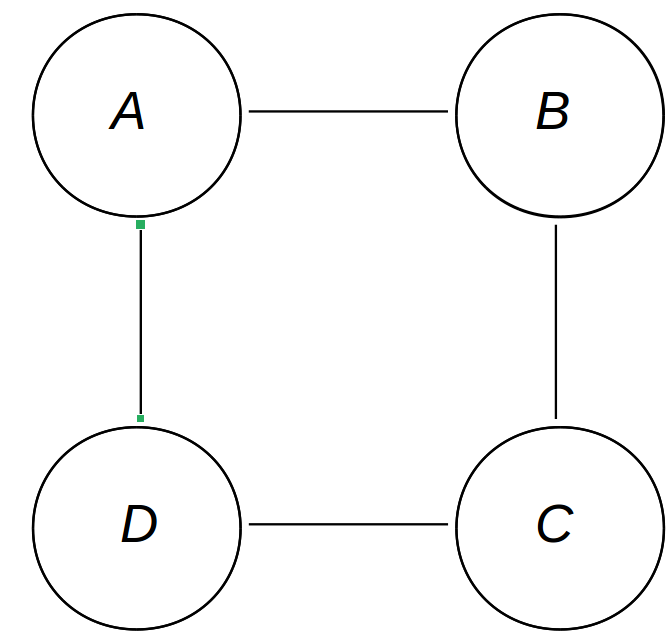
\includegraphics[width=\linewidth]{Figures/undirected_graph.png}
    \caption{Undirected graph}
  \end{subfigure}
  \begin{subfigure}[b]{0.3\linewidth}
    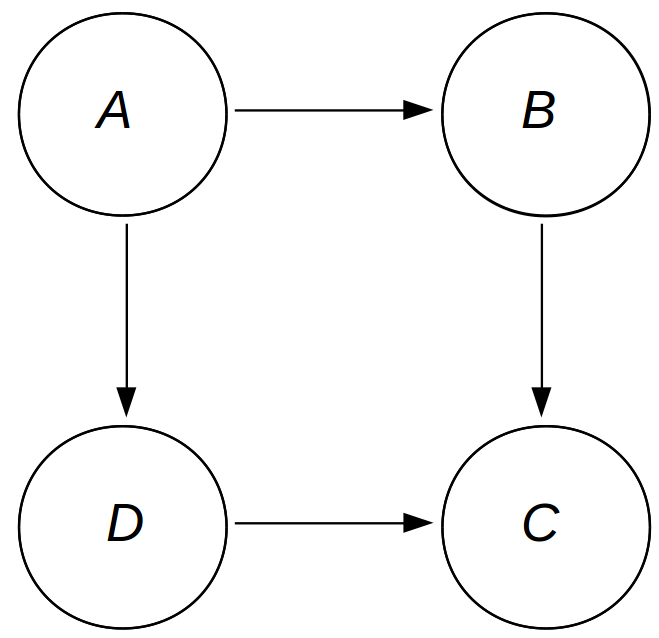
\includegraphics[width=\linewidth]{Figures/directed_graph.png}
    \caption{Directed graph}
  \end{subfigure}
  \caption{}
  \label{fig:comGraphs}
\end{figure}
\section{Bayesian PGMs}
A system with uncertainty can be modeled with a Bayesian network. Bayesian networks consists out of a set of nodes and directed edges. Nodes represent RVs($X_1, ..., X_n$). Edges indicate the relationship between nodes.\\
Each node is associated with a conditional probability distribution.
\begin{equation}
X_i \sim p(X_i|Par(X_i))
\end{equation}
where $Par(X_i)$ indicates the parent of node $X_i$.\\
The CPD associated with each node can be written as a factor. A factor is a function that takes a number of random variables as arguments.
\begin{equation}
\phi_i(X_i, Par(X_i)) = p(X_i|Par(X_i))
\end{equation}
Where the scope of a factor is its' arguments
\begin{equation}
Scope\{\phi_i\} = \{X_i, Par(X_i)\}
\end{equation}
Figure \ref{fig:bays_pgm} is an example of a Bayesian network with seven nodes labeled from $a$ to $c$. Each node is associated with a CPD. Directed edges between nodes are indicated with arrows.
\begin{figure}[H]
  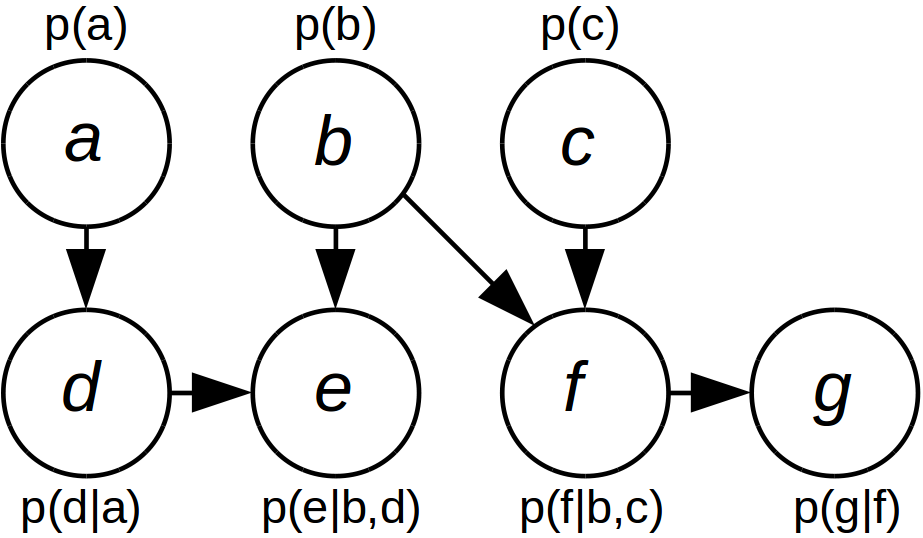
\includegraphics[width=0.6\linewidth]{Figures/bayesian_pgm.png}
  \centering
  \caption{Bayesian PGM}
  \label{fig:bays_pgm}
\end{figure}
\subsubsection{Chain Rule for Bayesian Networks}
The joint probability density distribution of all the variables in a Bayesian network can be found by finding the product of all the CPDs associated with nodes. (Koller and Friedman~\citep{koller})
\begin{equation}
p(X_1, ..., X_n) = \prod_i p(X_i|Par(X_i))
\end{equation}
Applying the Chain Rule to the Bayesian network in Figure \ref{fig:bays_pgm}
\begin{equation}
\begin{split}
p(a,b,c,d,e,f,g) & = p(a)p(b)p(c)p(d|a)p(e|b,d)p(f|b,c)p(g|f)\\
& = \phi_a(a)\phi_b(b)\phi_c(c)\phi_d(d,a)\phi_e(e,b,d)\phi_f(f,b,c)\phi_g(g,f)
\end{split}
\end{equation}
A marginal PDF of a subset of variables can be found by integrating over the remaining variables.
\begin{equation}
p(a,b,c) = \int\int\int\int p(a,b,c,d,e,f,g)dd\ de\ df\ dg
\end{equation}
\section{Cluster graphs}
After a Bayesian network has been constructed, it must be possible to reason about RVs in the network. Various methods can be used to inference a Bayesian network, one method is to construct a cluster graph. The cluster graph consists of clusters and undirected edges.\\Clusters are subsets of variables and can be formed by grouping factors together.\\
\begin{equation}
\bm{C}_i \subseteq \{X_1, ..., X_n\}
\end{equation}
The undirected edges between clusters are called sepsets and are responsible for passing messages between clusters. A sepset between two clusters contains information about variables that are common to both clusters.
\begin{equation}
\bm{S}_{i,j} \subseteq \bm{C}_i \cap \bm{C}_j
\end{equation}
There are multiple ways to construct clusters, but it should adhere to two requirements specified Koller and Friedman~\citep{koller}.\\
\textbf{1. Family Preservation}\\
Every factor $\phi_k$ in a set of factors $\Phi$ should be accommodated by a cluster.
\begin{equation}
Scope[{\phi}_k] \subseteq \bm{C}_i
\end{equation}\\
\textbf{2. Running Intersection Property}\\
There exists an unique path connecting a pair of clusters containing the same variable $X$, and every cluster and sepset along the path also contain $X$. This path allows clusters to share their beliefs of $X$. In other words, for any variable $X$, the set of sepsets and clusters containing $X$ form a tree~\citep{koller}. This prevents feedback loops and thus counters the phenomena where cluster's reinforce their own beliefs of variables.\\
Figure \ref{fig:bays_pgm} is updated in Figure \ref{fig:cluster_bound} where CPDs is replaced with factors and possible cluster boundaries are indicated with dashed rectangles. Note that there are other ways to construct the cluster graph.
\begin{figure}[H]
  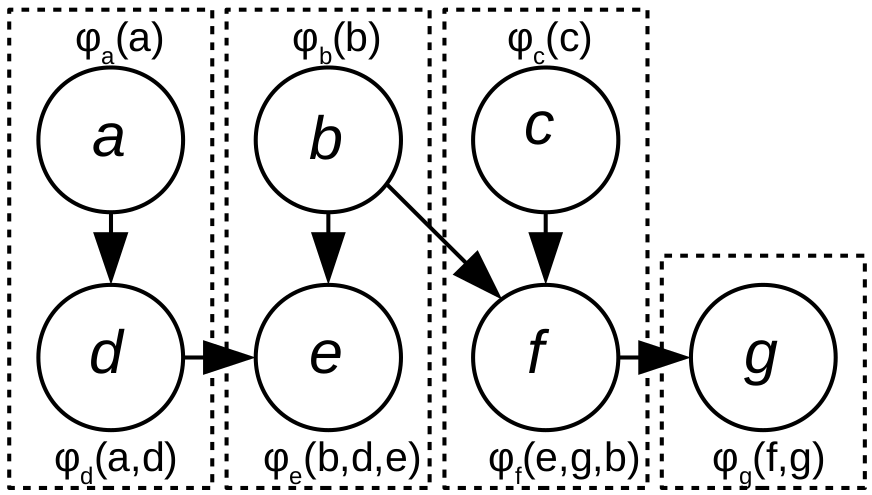
\includegraphics[width=0.6\linewidth]{Figures/cluster_divisions.png}
  \centering
  \caption{Bayesian PGM with cluster boundaries}
  \label{fig:cluster_bound}
\end{figure}

The initial belief of a cluster can be calculated by finding the product of all the factors inside the cluster.~\citep{koller}
\begin{equation}
\psi_i(C_i) = \prod_{k}\phi_k
\end{equation}
Figure \ref{fig:cluster_bound} is updated in Figure \ref{fig:clustergraph}. Clusters are indicated by ellipsis. Initial beliefs are calculated and shown inside the ellipsis. Sepsets are indicated by rectangles.\\
\begin{figure}[H]
  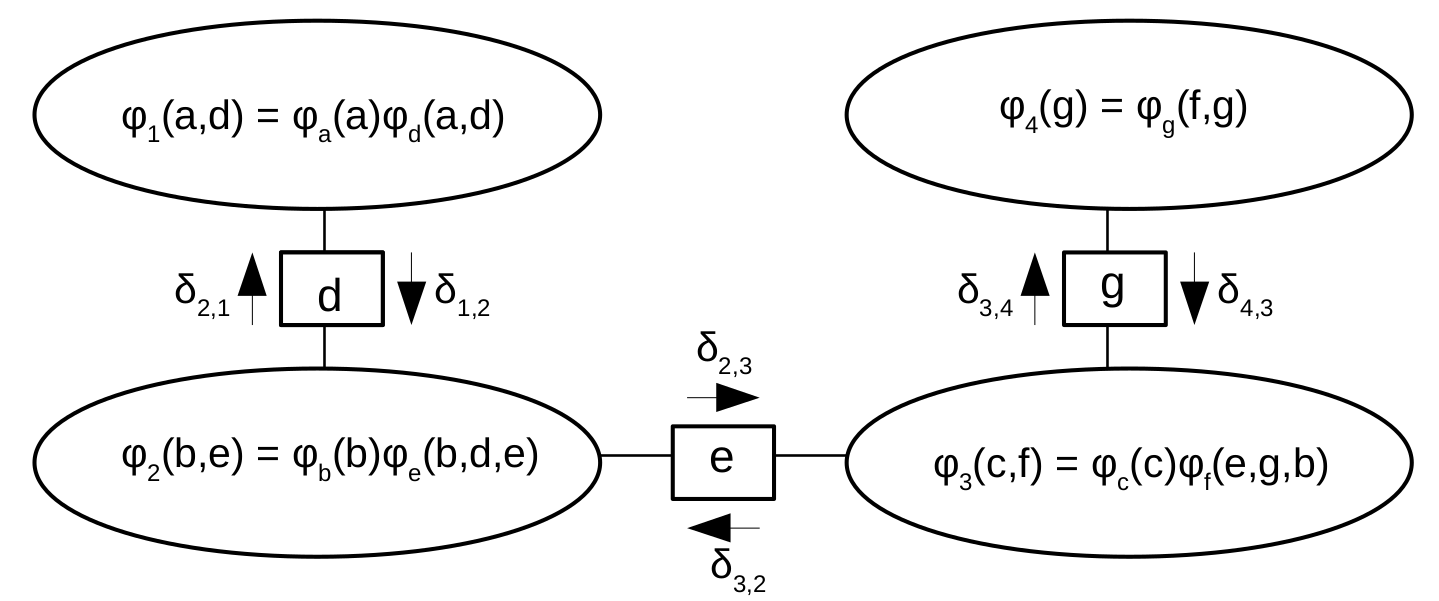
\includegraphics[width=\linewidth]{Figures/clustergraph.png}
  \centering
  \caption{Cluster graph}
  \label{fig:clustergraph}
\end{figure}
\section{Message Passing}
Clusters can share beliefs of common variables with messages passing. Messages are associated with sepsets. An outgoing message of a cluster can be calculated by multiplying the cluster with all the incoming messages and then integrating over the variables that are not in the sepset.
\\Thus, messages can be calculated accordingly~\citep{koller}
\begin{equation}
\delta_{i\to j}(\bm{S}_{i,j}) = \int_{\bm{C}_i - \bm{S}_{i,j}}\psi_i \times \prod_{k\ne j} \delta_{k\to i}(\bm{S}_{k,i})
\end{equation}
Applying to the cluster graph in Figure \ref{fig:clustergraph}
\begin{equation}\label{eq:del12}
\delta_{1,2}(d) = \int_a \psi_1(a,d)da
\end{equation}
\begin{equation}
\delta_{2,3}(b) = \int_d \int_e \delta_{1,2}(d)\psi_2(b,d,e)dd\ de
\end{equation}
\begin{equation}
\delta_{3,4}(f) = \int_b \int_c \delta_{2,3}(b)\psi_3(b,c,f)db\ dc
\end{equation}
\begin{equation}
\delta_{4,3}(f) = \int_g \psi_4(f,g)dg
\end{equation}
\begin{equation}
\delta_{3,2}(b) = \int_c \int_f \delta_{4,3}(f)\psi_3(b,c,f)dc\ df
\end{equation}
\begin{equation}
\delta_{2,1}(d) = \int_b \int_e \delta_{3,2}(b)\psi_2(b,d,e)db\ de
\end{equation}
Sometimes the value of certain variables in a PGM are known. This is known as evidence of a RV. If there is evidence of a RV, the evidence is available for entire the PGM and the RV itself doesn't appear in the PGM anymore. Evidence is indicated by a capital letter, thus $X$ is evidence of the RV $x$. Evidence is used to reduce PDFs, before calculating outgoing messages. Therefore RVs with evidence is left out of the integral when calculating messages.\\
In equation a message, containing RV $y$, is calculated. Evidence of $x$ is available and is indicated as $X$. The evidence of $x$ is used to reduce the cluster $\psi_i$. After $\psi_i$ has been multiplied with all other incoming messages, the result is integrated, but only over $z$.
\begin{equation}
\delta_{i\to j}(y) = \int_{z}\psi_i(x = X, y, z) \times \prod_{k\ne j} \delta_{k\to i}(\bm{S}_{k,i})
\end{equation}
After all the incoming messages of a cluster have been determined, the belief of a cluster can be calculated by multliplying the cluster's initial belief with all of the incoming messages, and normalizing the end result. Koller and Friedman~\cite{koller} specifies this as
\begin{equation}
\beta_i(\bm{C}_i) \propto \psi_i \times \prod_{k} \delta_{k \to i}(\bm{S}_{k,i})
\end{equation}
\section{Summary}
Bayesian networks consists of factors and directed edges.\\
Cluster graphs can be constructed by grouping factors.\\
Clusters in a cluster graph are connected by sepsets.\\
Adjacent clusters pass information to each other about variables in sepset.\\
Outgoing messages can be calculated with equation 4.11.

\chapter{Localisation using Probabilistic Graphical Models}
\section{Linear localisation}
\section{Non-linear localisation}
\subsection{Taylor series expansion}
\subsection{Unscented transform}
\subsection{Monte Carlo integration}

\backmatter
\bibliography{mybib}{}

\end{document}\grid
